\graphicspath{{./assets/}}
\setcounter{mtc}{3}
\chapter{1st Sprint: Maintenance of existing resources  }
\fancyhead[R]{\ungaramond\small\textbf{Chapter III. 1st Sprint: Maintenance of existing resources }}
\minitoc
\newpage


\section*{Introduction}
The first sprint was dedicated towards exploring the existing services and resources, performing some minor changes and putting in place a backup strategy.

\section{Sprint backlog :}

\begin{longtable}[H]{|m{1.5cm}|m{3cm}|m{1.5cm}|m{8cm}|}
\hline
{\textbf{EpicID}} & {\textbf{Epic}} & {\textbf{StoryID}} & {\textbf{Story}} \\
\hline
1 &  \raggedright Exploring assets.	& 1.1  & SCM structuring: service components need to be split into different repos. \\
\cline{3-4}
& & 1.2 &  	Keeping track of developed applications and their requirements \\
\hline
2  & Maintenance. &	2.1	 &  Rebuilding optimized containers for developed applications. \\
\cline{3-4}
& & 2.2 & Backup of existing data on current infrastructure in S3 containers.\\
\hline
\caption{1st sprint Backlog}
\end{longtable}

\section{Maintenance operations}

In this sprint, we have assembled standalone self-hosted services into a single stack of upgraded container versions in order to provide better visibility of workloads. A container management platform was then added to this stack to improve on operability. 
The following figure is the deployment diagram of the resulting docker-compose stack:

 \begin{figure}[H] 
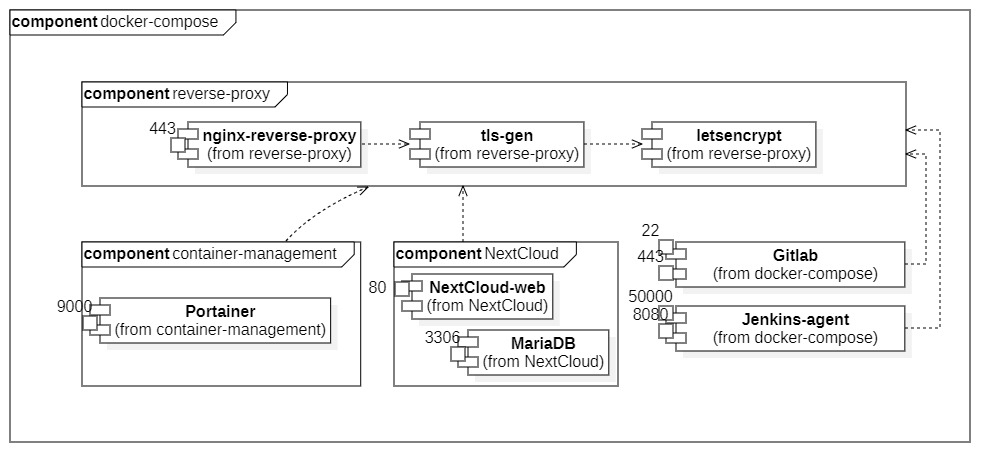
\includegraphics[width=1.0\textwidth,angle=00]{assets/f9.jpg}
\caption{PaaS infrastructure}
\label{fig:f9}
\end{figure}

The stack includes the following services: 
\begin{enumerate}
\item Nginx reverse proxy: An HTTP server that acts as a reverse proxy for the other services in the stack. It is responsible for routing traffic to the correct service based on the URL and handling HTTPS encryption. It recognizes labels configured in the containers to route traffic and provide tls termination. 
\item TLS generator: A service that generates and renews TLS certificates using Let's Encrypt. It works with Nginx to provide HTTPS encryption for the other services in the stack. 
\item Let's Encrypt: A certificate authority that provides free TLS certificates. 
\item Portainer: A web-based management interface for Docker containers and services. 
\item Nextcloud: A cloud-based file sharing and collaboration platform. 
\item GitLab: A web-based Git repository manager, CI/CD pipeline tool, and issue tracker. 
\item Jenkins: An open source automation server that can be used to automate software build, test, and deployment processes. 
\end{enumerate}

Each service is defined in a separate Docker container and is configured using environment variables, volumes, and ports. The Nginx and TLS generator services depend on each other, and the Nextcloud, GitLab, and Jenkins services depend on the TLS generator for HTTPS encryption. 

This Docker Compose stack provides a scalable and easy-to-manage infrastructure for hosting multiple cloud-based services, all secured using HTTPS encryption and Let's Encrypt TLS certificates. 




\section{Application overview and SCM structuring}

Two main applications were in development during this project. We have recommended a better source code management strategy that resulted in separating services into different repos in order to optimize the container image creation process. The resulting deployment diagram Is as follows: 

 \begin{figure}[H]\centering
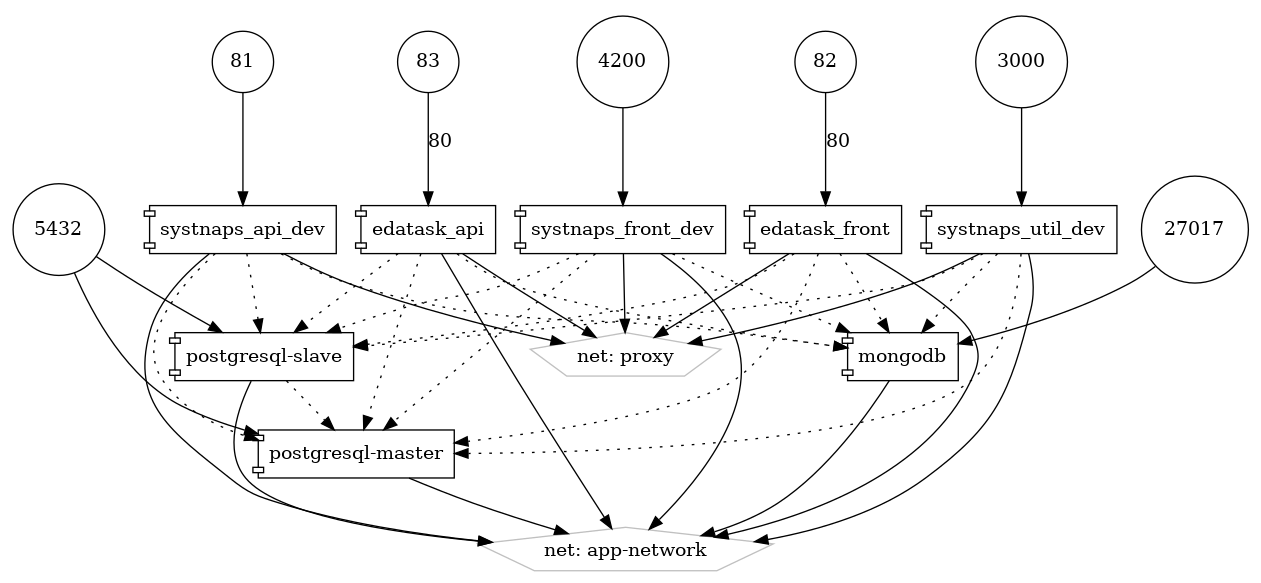
\includegraphics[width=1.0\textwidth,angle=00]{assets/f10.png}
\caption{ Deployment Diagram }
\label{fig:DeploymentDiagram}
\end{figure}

The stack includes the following services: 
\begin{enumerate}
\item Backend API: A Symfony\cite{Symfony} API that serves as the backend for the application. It is responsible for processing requests and returning data to the frontend. 
\item Frontend: An Angular\cite{Angular} web application that serves as the frontend for the application. It is responsible for displaying data and interacting with the backend API. 
\item HA PostgreSQL\cite{PostgreSQL}: A relational database management system that stores data for the application. It is used to store structured data for the backend API. 
\item Replicated MongoDB\cite{MongoDB}: A NoSQL database management system that stores data for the application. It is used to store unstructured data for the frontend. 
\item Nginx\cite{Nginx}: A web server that acts as a reverse proxy for the other services in the stack. It is responsible for routing traffic to the correct service based on the URL and handling HTTPS encryption. 
\end{enumerate}

The backend API, frontend, MongoDB and PostgreSQL are connected using the "app-network" network. All services are also connected to the "proxy" network where Nginx resides, enabling the reverse proxy detect labels and route traffic to the appropriate service based on the URL. 

\section*{Conclusion}
In this chapter, we covered several important practices such as structuring the SCM, keeping track of application requirements, rebuilding optimized containers, and backing up data. 

These practices help ensure that our infrastructure is up-to-date, secure, and efficient.  

The next step in the evolution of our infrastructure is migrating to a new self-managed Kubernetes cluster. 

This migration process will require careful planning, testing, and monitoring to ensure a smooth transition. 

Overall, maintenance is an ongoing process that needs to be carried out diligently to ensure the stability and availability of the infrastructure.

